\section{Choosing the lists before offers and after them}\label{sec:policy}
A platform that can recommend five programs per applicant has two opportunities to act. Before DA it knows the estimated chance of an offer at each program and the number of seats. Once tentative offers are issued, it also knows which students and seats remain available. The second observation changes what the platform can promise to an individual.
\subsection{How much predicted recovery does an extra place cost?}\label{sec:shortlist-frontier}
A platform need not choose between independent row rankings and an arbitrary coordinated assignment. Given a desired number $r$ of feasible placements, it can give up the smallest possible amount of predicted partner coverage. Let $u_j$ be the number of seats at program $j$, $q_i=\min(k,d_i)$ the number of recommendations for applicant $i$, and $s_{ij}$ a score on a common cardinal scale. When $s_{ij}$ is the probability that $j$ is $i$'s full-list partner, summing the displayed scores gives the predicted number whose partner is shown, without requiring independence across people. Write $D_0$ for rowwise top-$q_i$ and $\tau_i$ for the last retained score. Skip rows with no slots. Write $\nu(D)$ for the maximum number of applicants that the display can assign within the seat capacities.

\begin{theorem}[The price of visible capacity]\label{thm:capacity-frontier}
Suppose all applicants can receive a separately chosen list. For every $0\le r\le\nu(E)$ the minimum loss of total score from $D_0$, over quota-respecting displays $D$ with $\nu(D)\ge r$, is
\[
L(r)=\min_{A:\,|A|=r}\;\sum_{(i,j)\in A}(\tau_i-s_{ij})_+ ,
\]
where $A$ ranges over feasible assignments respecting program capacities. The nonnegative marginal losses $L(r+1)-L(r)$ are nondecreasing. For one recommendation per applicant, $r$ is also a lower bound on the number placed by DA under \emph{every} strict preference and responsive priority order on the display.
\end{theorem}
\begin{proof}
Any admissible display contains an assignment of size $r$. Each of its rows containing an assigned edge $(i,j)$ loses at least $(\tau_i-s_{ij})_+$ relative to its best list. Distinct assigned edges use distinct applicant rows, so these lower bounds add. Conversely, take a minimizing assignment. On each assigned row force its assigned edge onto the list and choose the best $q_i-1$ remaining edges. On every other row take its best list. This attains the sum, including when boundary scores tie.

Send $r$ units of flow from a source through applicants, admissible programs and a sink, with applicant arcs of capacity one and program-to-sink arcs of capacity $u_j$. Only applicant--program arcs carry the displayed replacement costs. Integral flow produces a minimizing assignment. The average of optimal flows of values $r-1$ and $r+1$ is feasible at value $r$. Integrality at that integer value gives $2L(r)\le L(r-1)+L(r+1)$. Deleting one assigned edge shows monotonicity. At quota one, every applicant with an option makes exactly one proposal. Each program holds the smaller of its capacity and its number of applicants, exactly exhausting the display's feasible placement count.
\end{proof}

This uses a standard minimum-cost flow primitive \citep{ahuja1993flows}. Flow-based recommender post-processing previously traded relevance against item exposure counts \citep{antik2017}. Here the constraint is the number of \emph{different people who could simultaneously be assigned}. Showing the same available programs to many applicants can meet an exposure target while leaving too few seats for those particular people. The cost of forcing an edge is its opportunity cost in that person's list. Choosing a maximum-weight assignment on the unadjusted scores optimizes a different objective.

\paragraph{What the platform can guarantee without knowing preferences.}
Under responsive priorities, every stable matching is maximal: an unmatched applicant cannot see a program with a vacant seat. Conversely, if both strict orderings are unknown, every maximal assignment can occur under applicant-proposing DA. To realize one, put each assigned program first on its holder's list and put all designated holders first in its program's priority. Unassigned applicants only see full programs by maximality. Thus the graph alone certifies exactly the size of its smallest maximal assignment in the worst case. In particular it certifies at least $\lceil\nu(D)/2\rceil$: expand each program into its seats. Each edge of a maximum matching either belongs to the maximal matching or meets one of its matched endpoints. Each edge of the maximal matching accounts for at most two edges of the maximum matching. The factor is sharp already at quota two: applicant $a$ sees $x,y$ in that order, $b$ sees only $x$, and $x$ prioritizes $a$. Both can be assigned, but only $a$ is placed by DA. Computing the exact worst-case size is NP-hard for unit-capacity bipartite graphs of maximum degree three by the minimum maximal matching result of \citet{yannakakis1980}. Deciding whether all strict profiles place at least $r$ is coNP-complete, since a smaller maximal assignment certifies failure. These worst-case statements allow preference and priority orderings to vary. For observed orders the realized DA allocation is determined and can be computed directly.


\paragraph{Applying the capacity requirement to national admissions.}
Starting from the rank-informed network's five suggestions, 177,963 applicants could simultaneously receive a displayed program under some feasible assignment. The full submitted graph allows 179,274. We kept the trained network fixed and required the display to close one quarter, one half, three quarters or all of this 1,311-seat gap. The predicted number of covered offers fell by only 20.19 at the maximum target. Yet program priorities and applicant choices matter: only 19 additional applicants were placed by DA. Twenty-nine previously unmatched people gained and ten previously matched people lost a place relative to the unmodified top five. Even though we allowed more simultaneous assignments, no extra applicant was placed at either of the two intermediate targets below three quarters. Table~\ref{tab:capacity-policy} gives the full sequence.

\begin{table}[ht]\centering\small
\caption{Same rank-informed network and same 189,399 university applicants. A feasible assignment witnesses each capacity target. Predicted loss is the sum of the covered probability mass sacrificed across applicants, in units of expected covered offers. The last column is DA's change in the number placed relative to the original model menus.}
\label{tab:capacity-policy}
\begin{tabular}{@{}lrrrr@{}}\toprule
Fraction of gap & Visible capacity & Displayed slots changed & Predicted loss & DA gain\\\midrule
None & 177,963 & 0 & 0 & 0\\
One quarter & 178,291 & 380 & 0.0025 & 0\\
One half & 178,619 & 740 & 0.1091 & 0\\
Three quarters & 178,947 & 1,285 & 1.9099 & 6\\
All & 179,274 & 2,132 & 20.1886 & 19\\\bottomrule
\end{tabular}\end{table}

We solved the capacitated min-cost flow using replacement costs rounded to billionths. The optima are exact for those integers. The difference from an optimum for unrounded scores is at most $r/10^9$ in total predicted coverage (less than 0.00018 here). We independently certified all eight positive-target integer objectives by matching each primal value to a feasible dual lower bound. A separate flow and cut certify each reported visible capacity. Reordering the flow arcs twice changed some optimal lists while giving the same 19 extra placements at the maximum target. With menus fixed, substituting 0\%, 25\%, 50\% or 75\% of published overbooking for the full amount gave placement gains of 48, 37, 16 and 21. The blind model's full-capacity display added 28 places at the published capacity. The rental simulations give a different scale: the exact repair raised ordinary-sample placement by 1.41 points in summer and 1.60 points in winter. The simple assignment anchor still achieved slightly higher DA placement at the same feasible capacity (Appendix~\ref{app:policy-detail}).

\subsection{One referral after tentative offers}\label{sec:residualreferral}
An applicant sees five programs, applies, and receives no offer. A clearinghouse can now observe which seats are still vacant. Suppose it can also see the applicant's eligible alternatives or ask which additional programs they would attend. How many people could receive a place with one additional referral each and all provisional contracts still feasible?

Let $D$ be the initial display, $M$ any stable matching on $D$, and $U$ the unmatched applicants. Program $j$ has integer capacity $c_j$ and $v_j=c_j-|M(j)|$ vacancies. Its fixed, strict priorities are responsive: given any set of acceptable applicants, it prefers to fill its capacity with the highest-priority members of that set. Construct a graph between $U$ and programs with $v_j>0$, keeping each mutually acceptable pair in the full feasible graph. Each such pair is hidden in $D$; otherwise it would block $M$. Assume $q_i=\min(k,d_i)$, where $k\ge1$ and $d_i$ is the applicant's feasible degree. Give program $j$ capacity $v_j$ in this graph and let $r$ be its maximum matching size.

\begin{theorem}[Vacancy referrals with a fixed quota]\label{thm:residualreferral}
At most $r$ initially unmatched applicants can be added to an allocation containing every original contract. This number is attainable with one display substitution for each of $r$ applicants and no change to any other list. Applicant-proposing DA on the resulting display places exactly the original recipients and those $r$ applicants and gives each original recipient a weakly preferred contract. If only a subset of the selected applicants agrees to its substitution, these same conclusions hold for that subset.
\end{theorem}
\begin{proof}
Any extension keeping $M$ intact can add at most $v_j$ people at each program. Its added pairs therefore form a matching in the residual graph. Conversely, take any residual matching $A$. Show each selected applicant their assigned program, dropping their least preferred displayed program to keep their quota. Under the usual rule $q_i=\min(k,d_i)$ the existence of a hidden feasible pair implies $d_i>k$; if the platform instead allows an unused slot, it can use that slot.

Write $W=M\cup A$. Each newly displayed pair belongs to $W$. On an old displayed pair the applicant's assignment has weakly improved relative to $M$. An originally full program has exactly its old occupants in $W$. At an originally slack program every applicant with an old displayed edge already weakly preferred their assignment under $M$ to that program, by stability. Thus no displayed pair blocks $W$, and all partners remain visible. Applicant-proposing DA weakly dominates $W$ for every applicant, and invariance of the matched applicant set across stable outcomes gives exactly its recipient set. For opt-outs delete the relevant edges from $A$ and keep their original menus; the proof applies to the remaining residual matching.
\end{proof}

This is a certificate for an extension that leaves the original contracts available as a stable witness. DA may improve an incumbent's partner. Moving incumbents on their own newly revealed edges could create further placements, an objective outside this bound. A prior year's predicted vacancies do not certify an extension of today's offers. The stability guarantee is relative to the revised display. The institution needs the ability to direct individual referrals or to reserve them, alongside an accepted list of otherwise undisplayed choices. Publicly announcing every vacancy can induce several people to chase the same seat. \citet{lepesure} simulates a Chilean school mechanism that helps unassigned applicants find previously unlisted nearby schools and runs a targeted residual submarket preserving earlier allocations. Our question concerns previously submitted options displaced by a quota. We compute the maximum contract extension under that restriction and certify a full-market DA rerun after an individual substitution or opt-out. Other work studies efficiency after cancellations and repeated general admission rounds \citep{feigenbaumreallocation,gradualschool}.

The graph also determines whether access has to be rationed among people with a feasible vacancy. For $L$ a subset of unmatched applicants with a residual edge and $N(L)$ their neighboring programs, at most $\sum_{j\in N(L)}v_j$ members of $L$ receive one of those seats. The largest deficit $|L|-\sum_{j\in N(L)}v_j$ is exactly the number of applicants with a residual edge left out by a maximum flow. A minimum cut provides a witness. If a group of applicants is to receive priority among maximum-size extensions, solve a maximum-weight residual matching with weight $n+1+\mathbf{1}\{i\text{ belongs to the group}\}$ on every eligible edge. The integer $n$ bounds the number of applicants. This gives the most group members who can be served at the maximum total; the same witness proof applies.

\paragraph{Who can actually use a vacancy?}
After the rank-informed university menus cleared, 30,866 applicants had no placement and 21,061 seats remained vacant. Only 160 of the unmatched applicants had submitted any eligible program with a vacancy. Among these, 24 shared just 11 reachable seats. That bottleneck accounts for all 13 people the residual matching could not place. The coordinated referrals placed 147 additional applicants without worsening any incumbent's assignment. In contrast, letting everyone add their own favorite vacancy placed 156 new applicants but displaced 11 incumbents. Running DA in a separate residual market placed 143 with no losses. The median referred option in the maximum extension ranked fourteenth on the applicant's original list. If the referral must be among the applicant's own first five choices, the maximum falls to four. At a rank limit of ten it reaches 61. Each selected applicant may decline. We assume full take-up for the reported volume comparison.

\begin{figure}[ht]\centering
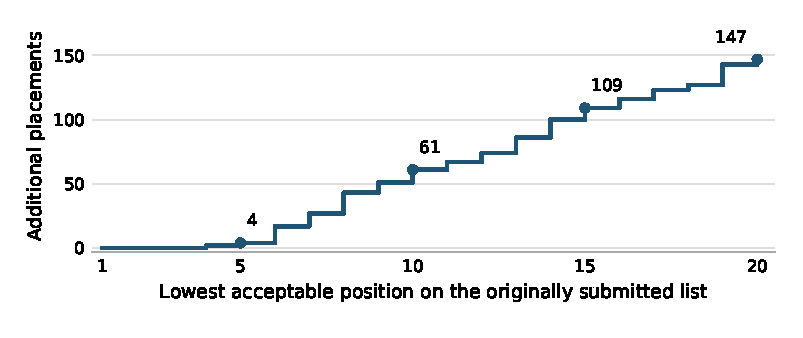
\includegraphics[width=.78\linewidth]{figures/referral-rank.pdf}
\caption{How far down their original lists would applicants have to go? Each point is the maximum number of additional placements compatible with retaining all provisional contracts after the rank-informed university model. A rank limit of five admits four new placements; a limit of twenty admits 147. The horizontal axis is a scenario about acceptable options, not observed take-up.}
\Description{An increasing staircase has 4, 61, 109 and 147 additional placements when referrals may reach original ranks 5, 10, 15 and 20.}
\label{fig:referral-rank}\end{figure}

The attainable gain depends on what the original rule already achieved. Starting from each applicant's first five reported programs allowed 7,268 additional placements in 2026. Starting from the rank-blind network allowed 61. In the 2,304 simulated rental markets, coordinated referrals added 9,749 placements against 5,761 when each applicant chose their favorite vacancy independently. Giving lower-income applicants priority among equally large extensions increased their additional placements from 3,059 to 3,155 with the same total. These are counts across ordinary and enriched simulation draws. Appendix~\ref{app:policy-detail} gives the designs separately and shows what breaks when tentative offers are forecast rather than observed.
